\documentclass[a4paper,11pt,twocolumn]{article}
\usepackage[a4paper]{geometry}
\geometry{textwidth=480pt, textheight=674pt}
\renewcommand{\vec}[1]{\mathbf{#1}}
\usepackage{ragged2e}
\usepackage{multicol}
\usepackage{fixltx2e}
\usepackage{graphicx}
\usepackage{url}
\graphicspath{{images/}}
\usepackage{amsmath}
\usepackage{gensymb}
\usepackage{listings}
\usepackage{lstautogobble}
\usepackage[font={small,it}]{caption}
\usepackage{tabu}
\usepackage[utf8]{inputenc}
\usepackage[english]{babel}
\setlength{\parindent}{4em}
\setlength{\parskip}{1em}
\renewcommand{\baselinestretch}{1}

\begin{document}
	\setcounter{secnumdepth}{0}
	%\doublespacing
	\pagenumbering{arabic}
	\centering
	\onecolumn
	
	\title
	\maketitle{\huge\bfseries Board Health Monitoring System for Phase II ATCA Service Card}
	
	\emph{David Monk -- 00928791}
	
	Word count: 1851
	
	\twocolumn
	%\onehalfspacing
	
	\justify
	\section{Abstract} 
	This report summarises the work done during the Summer 2017 UROP scheme. A COM-Express module mounted on the ATCA service card was used to communicate with other I\textsuperscript{2}C components on the board to assess their health and configuration. This data was then synchronised with an external master database using couchDB, a NoSQL database format. 
	\section{Introduction} 
As part of the upgrades for Phase II of CMS, the MP7 trigger cards are set to be replaced by a new card with the ATCA[cite] form factor. The larger card area allows for greater customisability and scope for on-card control hardware.

	The COM-Express is a compact computer-on-module (COM) form-factor PC, designed for embedded systems. The Adlink nanoX-BT, chosen for the test service card contains either an Intel\textregistered Atom\textsuperscript{TM} or Intel\textregistered Celeron\textregistered CPU, up to 4GB RAM and full Ethernet, PCIe and USB support[cite]. CentOS 7, a Linux/UNIX operating system, was chosen to be installed, in line with CERN standards. 

	With such processing power on the card itself, a proposal for the system management model for the service card is to allow for semi-autonomous operation, removing the need for a rack PC (see figure ()). The overall proposed structure was to have a single master database on an external machine which contains register data from all cards, as well as configuration files for each card. Any changes to configuration files would then be pushed to the card in question, whereby the changes would be made to appropriate registers. For more urgent changes, local feedback loops could be implemented, removing all dependency on a master database and decisions to be made at a COM-Express level. Register data would still be fed to the master database, allowing for these decisions to be supervised and analysed by an external PC. 
	
	\section{Building the System} 
	\subsection{I\textsuperscript{2}C Stack} 
	The I\textsuperscript{2}C protocol is a de facto standard for multi-master, multi-slave serial communication on a circuit board[cite]. The two-wire bus allows for simple design while the bit-rate is easily sufficient for monitoring and configuration. The aim behind the I\textsuperscript{2}C was to build a type-safe library from database to physical register on the board. In doing so, each property on the board would comprise of a value and, where applicable, an associated unit. If the unit given by the database was not valid, the property to be written would simply not be accepted by the software. 

	\begin{figure}
		\centering
		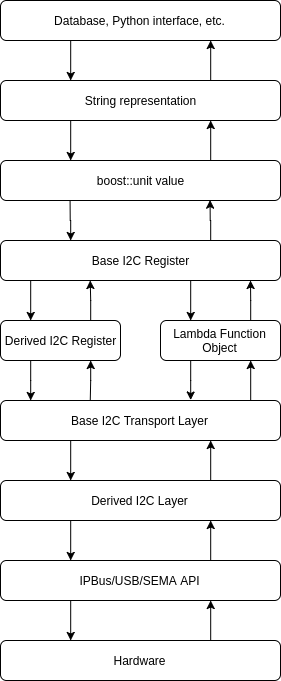
\includegraphics[width=\columnwidth]{stack-diagram}
		\caption{Stack diagram for I\textsuperscript{2}C code. Type-safety checking is conducting within the I2CRegister layer.}
	\end{figure}

	Figure () shows a basic stack diagram for the software. At the top-level, the stack accepts and outputs strings as its way of communicating between the database. Heavy use is then made of Boost libraries, in particular: Variant, Unit and the Qi parser. This allows the string to be converted to a \verb|boost::unit|, which is then passed onto the \verb|I2CRegister| class. The \verb|I2CRegister| class implements the core read/write functionality for accessing the I\textsuperscript{2}C register as well checking the type-safety of the value that is passed. For simple registers, i.e. those whereby the value is simply converted to a byte and then written, a lambda function implements all of the type checking and I/O. More complex properties, for instance those which span multiple registers or specific bits within a register, the \verb|I2CRegister| base class was extended to allow for further functionality. 
	
	The Adlink COM-Express contains scope for the Smart Embedded Management Agent (SEMA) utilities, including a library for I\textsuperscript{2}C access. Function calls for reading and writing to an address, including an offset, greatly simplified the bridge between COM-Express and card components. For that reason, only a light wrapper was required to interface with the type-safe variables. Furthermore, the framework was designed to be independent of the I\textsuperscript{2}C standard, thus allowing for other standards such as FTDI and PCI translation to also be implemented. 

	During testing and deployment of the code, a number of problems arose. Firstly, the I\textsuperscript{2}C architecture of the service card (see figure ()) was more complex than a simple serial bus, meaning that a number of configuration steps had to be implemented before the code could communicate with a given component. These steps were compounded by an address conflict between the arbiter and fanout, resulting in the latter being unconfigurable. This problem was resolved by changing the address by manually pulling up pin 2 on the fanout, thus changing the address. The arbiter was also initially in a constant external reset state which was again fixed by manually pulling up the appropriate pin. 
	
	The only communicable component on the service card was the PCI clock buffer (Si53106) used to generate a reference clock for the PCIe output lanes. Accessible registers within this component included IDs as well as PLL mode and the output enable. Although limited, these properties were sufficient to test the stack and further database structures. An ethernet PHY (VSC8211) was also present on the board, however this was not communicable, an issue which is as yet unresolved. With the next revision replacing the arbiter and fanout with a programmable FPGA, which should simplify configuration, it may be easier to isolate the issue. 
	
	\subsection{Distributed Database} 
	NoSQL style databases, such as couchDB and mongoDB, have a number of significant advantages over conventional SQL standards. The main benefit is the document system for storage, compared to a relational database. The loss in query performance is compensated by complete flexibility in the contents of each document. Each document is a separate entity and thus consistency is not a requirement for the standard. Furthermore, couchDB employs a version control style of databasing, in the sense that local databases can be ``pushed" to a master external server. Conflicts when merging databases are resolved by a unique revision number associated with each document. If a document is changed, so does this revision number, ensuring that databases can only be merged if revision numbers match for each document. 

	For the test system, a couchDB server was set up on each test card, as well as a master database on a separate computer. Each card stored a local cache of register data before also pushing its contents to the master database. Each time the registers were polled, a new document was created on the local database, with a timestamp as ID. 

	Of the registers available through I\textsuperscript{2}C, some changed regularly (e.g. temperature or voltage), whilst others remained constant. Each property was thus categorized as either ``active" or ``static". Active registers were polled every 5 seconds, ensuring any changes were suitably recorded. Static registers were only polled once per hour and if the value had changed. 
	
	In order to reduce the data footprint on each local card, any data taken over an hour previously was deleted hourly. This, along with other operations such as polling static registers and checking for updates to configuration files, was performed on separate threads to the main active thread. The deletion operation had a significant time overhead and thus would have affected other functions if performed in a serial manner. This was trivially implemented using the \verb|C++11| threading library and a proprietary couchDB wrapper around \verb|libcurl| for the HTTP calls. 
	
	The stability of the code was tested over two and a half days, producing 44,919 documents in the master database for one card. The overall size of the data is 326.8MB, resulting in an average size per document of 7.45KB. This is significantly greatly than the equivalent JSON file for an example document, which is only 494 bytes. This significant overhead is most likely attributed to the database also storing revision history for each document, as well as the current data.  

	As indicated by the JSON file equivalent, the data stored contained only a small number of points. For the complete ATCA card, this number will certainly rise significantly, increasing the size of the document further. Thus, a yearly lower bound for the data produced by one card would be approximately 44.8GB. Scaled across a number of racks containing in the order of 500 cards, this number rises to 21.9TB of data. While incomparable to the volume of data produced by CMS itself, it is still significant and warrants further research into compacting the data. One such method could be to build a differential database, whereby only the changes to properties were recorded at a given time. While this would reduce the footprint for generally static registers, actively changing values would see a negligible change. 
	
	\subsection{Addendum: PDF Parsing} 
	As an aside from the I\textsuperscript{2}C work, a colleague requested a 400-page register list to be parsed into machine readable format. A number of approaches were considered, including an initial conversion to plain-text before parsing using pater recognition. The final approach, however was to make an initial parse into HTML code, whereby each table was converted into a HTML table. A number of irregularities in the parsing were solved through the magic of regular expressions and the work of Dr Andrew Rose, allowing the HTML to be further parsed into a Python \verb|ElementTree|[cite].  
	
	Once in this format, it was relatively trivial to extract appropriate rows and associated metadata in each table relating to a given register. JSON was used as an appropriate format for the data, mainly because of its portability and ease of parsing. 
	
	\section{Future work} 
	Much of the work conducted during this period was build a framework for further features to be added without the need to rewrite the entire framework. The architecture of the I\textsuperscript{2}C stack allows for a new bus, device or register to be added by simply modifying the \verb|unordered_map| which contains all the required data for the board. 
	
	The scalability of the database is currently untested, however the scope of the couchDB for concurrent calls to the master database should be sufficient according to its specifications. Confirming this would be possible by filling a crate with service cards, all communicating over the backplane, and thus having a local network over which the master database could also be connected. Although a local network is not a requirement for couchDB, this setup would be more representative of the final product. 
	
	\section{Conclusion} 
	The work conducted here will hopefully provide a contribution to the combined effort within the common hardware group at CMS towards a final ATCA standard card in time for the scheduled upgrade in 2022. While some work, such as that on configuring the I\textsuperscript{2}C Arbiter, will become redundant in the next iteration of service card, a number of valuable lessons were learnt in building the framework which can be then applied for future versions. 

	On a personal note, my programming skills, particularly in C++, have improved immeasurably during my time working on this project. Furthermore, I have gained a far better understanding of the UNIX operating system at a lower level than before, in order to debug issues that arose during testing. At a hardware level, I gained significant experience in debugging a number of systems, including I\textsuperscript{2}C and the ethernet switch (the latter conducted mainly at the CERN campus). 
	
	I would like to thank the High Energy Physics group at Imperial College, in particular Dr Andrew Rose, for the opportunity to conduct this work.
	
	\bibliography{bib}
	\bibliographystyle{ieeetr}
	
\end{document}
